\documentclass[11pt]{beamer}
\usetheme{CambridgeUS}
\usepackage[utf8]{inputenc}
\usepackage{amsmath}
\usepackage{amsfonts}
\usepackage{amssymb}
\usepackage{graphicx}
\usepackage{pgfpages}
\usepackage{framed}
\usepackage{xcolor}
\usepackage[most]{tcolorbox}
\usepackage{soul}
\usepackage{empheq}

% The replacement character � (often displayed as a black rhombus with a white
% question mark) is a symbol found in the Unicode standard at code point U
% +FFFD in the Specials table. It is used to indicate problems when a system 
% is unable to render a stream of data to a correct symbol.[4] It is usually 
% seen when the data is invalid and does not match any character. For this 
% reason we map explicitly this character to a blanck space.
\DeclareUnicodeCharacter{FFFD}{ }

\newcommand*{\itemimg}[1]{%
  \raisebox{-.3\baselineskip}{%
    \includegraphics[
      height=\baselineskip,
      width=\baselineskip,
      keepaspectratio,
    ]{#1}%
  }%
}

\newtcbox{\mymath}[1][]{%
    nobeforeafter, math upper, tcbox raise base,
    enhanced, colframe=blue!30!black,
    colback=blue!10, boxrule=1pt,
    #1}

\newcommand{\highlight}[1]{%
  \colorbox{yellow!100}{$\displaystyle#1$}}

\author{Giovanni Della Lunga\\{\footnotesize giovanni.dellalunga@unibo.it}}
%\title{3 - Introduction to Deep Learning}
\title{3 - Introduction to Natural Language Processing}
%\title{7 - Classification for Text Analysis}
%\title{8 - Clustering for Text Similarity}
\subtitle{} % (optional)
\setbeamercovered{transparent} 
\institute{Advanced Machine Learning for Finance} 
\date{Bologna - April-May, 2022} 

\begin{document}

\begin{frame}
\titlepage
\end{frame}

\AtBeginSection[]
{
  %\begin{frame}<beamer>
  %\footnotesize	
  %\frametitle{Outline}
  %\begin{multicols}{2}
  %\tableofcontents[currentsection]
  %\end{multicols}	  
  %\normalsize
  %\end{frame}
  \begin{frame}
  \vfill
  \centering
  \begin{beamercolorbox}[sep=8pt,center,shadow=true,rounded=true]{title}  	\usebeamerfont{title}\insertsectionhead\par%
  \end{beamercolorbox}
  \vfill
  \end{frame}
}
\AtBeginSubsection{\frame{\subsectionpage}}

% INSERT HERE

%---------------------------------------------------------------------------------------------------
\section{What is NPL (Natural Language Processing)?}
%---------------------------------------------------------------------------------------------------
\begin{frame}{Introduction	}
	\begin{itemize}
		\item Natural language is what people use to communicate with each other. Unlike formal languages (e.g. programming languages), which are defined by strict rules, natural language is flexible, contextual, and evolving. 
		\item As a result, natural language is not as straightforward for a computer program to process as a script written in a language like Java, Python, or SQL. 
		\item When we talk about Natural Language Processing (or \textbf{NLP} for short), we are talking about the ways in which we can use computers to process and interact with human language.
	\end{itemize}
\end{frame}
%..................................................................
\begin{frame}{Introduction: What is NLP ?}
	\begin{itemize}
		\item Having an insight into what people are talking about can be very valuable to financial traders. 
		\item NLP is being used to track news, reports, comments about possible mergers between companies, everything can then be  incorporated into a trading algorithm;
		\item Banks can determine what customers are saying about a service or product by identifying and extracting information in sources like social media. 
		\item This sentiment analysis can provide a lot of information about customers choices and their decision drivers.
	\end{itemize}
\end{frame}
\begin{frame}{Introduction: What is NLP ?}
\textbf{Text Mining and Text Analysis}
	\begin{itemize}
		\item At some level, text analysis is the act of breaking up larger bodies of work into their constituent components - unique vocabulary words, common phrases, syntactical patterns - then applying statistical analysis to them;
		\item We will soon see that there are many levels to which we can apply our analysis, all of which revolve around a central text dataset: the \textbf{corpus}.
	\end{itemize}
\end{frame}
%..................................................................
\begin{frame}{Introduction: What is NLP ?}
\textbf{What is a Corpus}
	\begin{itemize}
		\item Corpora are collections of related documents that contain natural language. 
		\item A corpus can be large or small, though generally they consist of dozens or even hundreds of gigabytes of data inside of thousands of documents.
		\item A corpus can be broken down into categories of documents or individual documents.
	\end{itemize}
\end{frame}
%..................................................................
\begin{frame}{Introduction: What is NLP ?}
\textbf{What is a Corpus}
	\begin{itemize}
		\item Corpora can be \textbf{annotated}  \textit{meaning that the text or documents are labeled with the correct responses for supervised learning algorithms }, or \textbf{unannotated}, making them candidates for topic modeling and document clustering.
		\item  For example, one common type of annotation is the addition of tags, or labels, indicating the word class to which words in a text belong
	\end{itemize}
	\begin{center}
	\includegraphics[scale=0.5]{../7-pictures/04_basic_text_mining_picture_00.png}
	\end{center}
\end{frame}
%..................................................................
\begin{frame}{Introduction: What is NLP ?}
\textbf{Domain Specific Corpora}
	\begin{itemize}
		\item  The best applications tend to use language models trained on domain-specific corpora (collections of related documents containing natural language). 
		\item The reason for this is that language is highly contextual, and words can mean different things in different contexts. 
		\item For example, depending on context, the word \textbf{bank} can refer a place where you put your money, the side of a river, the surface of a mine shaft, or the cushion of a pool table! 
		\item With domain-specific corpora, we can reduce ambiguity and prediction space to make results more intelligible.
	\end{itemize}
\end{frame}
%..................................................................
%---------------------------------------------------------------------------------------------------
\subsection{The NLTK Package}
%---------------------------------------------------------------------------------------------------
\begin{frame}{NLTK Package}
\begin{columns}[T] % align columns
\begin{column}{.48\textwidth}
        \begin{itemize}
		\item The [Natural Language Toolkit](https://www.nltk.org/), or more commonly NLTK, is a suite of libraries and programs for symbolic and statistical natural language processing (NLP) for English written in the Python programming language.
		\item It was developed by Steven Bird and Edward Loper in the Department of Computer and Information Science at the University of Pennsylvania.
        \end{itemize}
\end{column}%
\hfill%
\begin{column}{.48\textwidth}
    %\fbox{
        \includegraphics[width=\linewidth]{../7-pictures/05_natural_language_processing_pic_0.png}
    %}
\end{column}%
\end{columns}
\end{frame}
%..................................................................
\begin{frame}{NLTK Package}
\begin{columns}[T] % align columns
\begin{column}{.48\textwidth}
        \begin{itemize}
		\item NLTK includes graphical demonstrations and sample data. 
		\item It is accompanied by a book that explains the underlying concepts behind the language processing tasks supported by the toolkit, plus a text book available also on line [here](https://www.nltk.org/book/)
        \end{itemize}
\end{column}%
\hfill%
\begin{column}{.48\textwidth}
    %\fbox{
        \includegraphics[width=\linewidth]{../7-pictures/05_natural_language_processing_pic_1.png}
    %}
\end{column}%
\end{columns}
\end{frame}
\begin{frame}{NLTK Package}
	\begin{itemize}
		\item The latest version is NLTK 3.3. It can be used by students, researchers, and industrialists. It is an Open Source and free library. It is available for Windows, Mac OS, and Linux. 
		\item You can install nltk using \textit{pip installer} if it is not installed in your Python installation. To test the installation:
		\item Open your Python IDE or the CLI interface (whichever you use normally)
		\item Type \textbf{\textit{import nltk}} and press enter if no message of missing nltk is shown then nltk is installed on your computer.
	\end{itemize}
\end{frame}
%..................................................................
\begin{frame}{NLTK Package}
	\begin{itemize}
		\item A \textbf{CorpusReader} is a programmatic interface to read, seek, stream, and filter documents, and furthermore to expose data wrangling techniques like encoding and preprocessing for code that requires access to data within a corpus. 
		\item A \textbf{CorpusReader} is instantiated by passing a root path to the directory that contains the corpus files, a signature for discovering document names, as well as a file encoding (by default, UTF-8).
		\item NLTK comes with a variety of corpus readers (66 at the time of this writing) that are specifically designed to access the text corpora and lexical resources that can be downloaded with NLTK.
	\end{itemize}
\end{frame}
%..................................................................
\begin{frame}{Corpus Reader}
	\textbf{PlaintextCorpusReader}. \textit{A reader for corpora that consist of plain-text documents, where paragraphs are assumed to be split using blank lines}.
	\begin{center}
	\includegraphics[scale=0.4]{../7-pictures/05_natural_language_processing_pic_2.png}
	\end{center}
\end{frame}
%..................................................................
\begin{frame}{Corpus Reader}
	\begin{itemize}
		\item \textbf{TaggedCorpusReader}. \textit{A reader for simple part-of-speech tagged corpora, where sentences are on their own line and tokens are delimited with their tag}. 
		\item \textbf{BracketParseCorpusReader}. \textit{A reader for corpora that consist of parenthesis-delineated parse trees}.
		\item \textbf{ChunkedCorpusReader}. \textit{A reader for chunked (and optionally tagged) corpora formatted with parentheses}.
		\item \textbf{TwitterCorpusReader}. \textit{A reader for corpora that consist of tweets that have been serialized into line-delimited JSON}.
		\item \textbf{WordListCorpusReader}. \textit{List of words, one per line. Blank lines are ignored}. 
		\item \textbf{XMLCorpusReader}. \textit{A reader for corpora whose documents are XML files}. 
		\item \textbf{CategorizedCorpusReader}. \textit{A corpus readers whose documents are organized by category}.
	\end{itemize}
\end{frame}
%---------------------------------------------------------------------------------------------------
\subsection{Text Preprocessing}
%---------------------------------------------------------------------------------------------------
%..................................................................
\begin{frame}{Tokenization}
	\begin{itemize}
		\item Tokenization Is the process of segmenting text into sentences and words. 
		\item In essence, it is the task of cutting a text into pieces called tokens, and at the same time throwing away certain characters, such as punctuation. 
	\end{itemize}
	\begin{center}
	\includegraphics[scale=0.55]{../7-pictures/05_natural_language_processing_pic_3.png}
	\end{center}
\end{frame}
%..................................................................
\begin{frame}{Stop Words Removal}
	\begin{itemize}
		\item In this process some very common words that appear to provide little or no value to the NLP objective are filtered and excluded from the text to be processed, hence removing widespread and frequent terms that are not informative about the corresponding text.
		\item Ex.: common language articles, pronouns and prepositions such as \textbf{and}, \textbf{ the} or \textbf{ to} in English.
		\item In many situations, stop words can be safely ignored by carrying out a lookup in a pre-defined list of keywords, freeing up database space and improving processing time.
		\item But \textbf{this is not always the case}.
	\end{itemize}
\end{frame}
%..................................................................
\begin{frame}{Stop Words Removal}
	\textbf{Be aware that}:
	\begin{itemize}
		\item There is no universal list of stop words!
		\item stop words removal can wipe out relevant information and modify the context in a given sentence. 
		\item For example, if we are performing a \textbf{sentiment analysis} we might throw our algorithm off track if we remove a stop word like \textbf{not}. 
		\item Under these conditions, you might select a minimal stop word list and add additional terms \textbf{depending on your specific objective}.
	\end{itemize}
\end{frame}
%..................................................................
\begin{frame}{Stemming and Lemmatization}
\textbf{Stemming}
	\begin{itemize}
		\item Stemming refers to the process of slicing the end or the beginning of words with the intention of removing affixes (lexical additions to the root of the word).
		\item Affixes that are attached at the beginning of the word are called \textbf{prefixes} (e.g. \textbf{ astro } in the word \textbf{ astrobiology}) and the ones attached at the end of the word are called \textbf{suffixes} (e.g. \textbf{ ful} in the word \textbf{ helpful}).
	\end{itemize}
	\begin{center}
	\includegraphics[scale=0.5]{../7-pictures/05_natural_language_processing_pic_4.png}
	\end{center}
\end{frame}
%..................................................................
\begin{frame}{Stemming and Lemmatization}
\textbf{Lemmatization}
	\begin{itemize}
		\item Has the objective of reducing a word to its base form and grouping together different forms of the same word. 
		\item For example, verbs in past tense are changed into present (e.g. \textbf{went} is changed to \textbf{ go }) and synonyms are unified (e.g. \textbf{ best } is changed to \textbf{ good }), hence standardizing words with similar meaning to their root. 
		\item Although it seems closely related to the stemming process, lemmatization uses a different approach to reach the root forms of words.
	\end{itemize}
\end{frame}
%..................................................................
\begin{frame}{Stemming and Lemmatization}

Typically a large corpus will contain many words that have a common root – for example: offer, offered and offering. Lemmatisation and stemming both refer to a process of reducing a word to its root. The difference is that stem might not be an actual word whereas, a lemma is an actual word. It’s a handy tool if you want to avoid treating different forms of the same word as different words. Let's consider the following example:
\begin{itemize}
	\item \highlight{\textbf{Stemming}}: considered, considering, consider → “consid”
	\item \highlight{\textbf{Lemmatising}}: considered, considering, consider → “consider”
\end{itemize}
\end{frame}
%..................................................................
\begin{frame}{Stemming and Lemmatization}
	\begin{itemize}
		\item Lemmatization resolves words to their dictionary form (known as lemma) for which it requires detailed dictionaries in which the algorithm can look into and link words to their corresponding lemmas.
		\item For example, the words \textbf{running }, \textbf{ runs }  and  \textbf{ ran }  are all forms of the word \textbf{ run }, so \textbf{ run} is the lemma of all the previous words.
	\end{itemize}
	\begin{center}
	\includegraphics[scale=0.5]{../7-pictures/05_natural_language_processing_pic_5.png}
	\end{center}
\end{frame}
%..................................................................
\begin{frame}{Stemming and Lemmatization}
	\begin{itemize}
		\item lemmatization is a much more resource-intensive task than performing a stemming process. 
		\item At the same time, since it requires more knowledge about the language structure than a stemming approach, it \textbf{demands more computational power} than setting up or adapting a stemming algorithm.
	\end{itemize}
\end{frame}
%..................................................................
\begin{frame}{Example}
\begin{columns}[T] % align columns
\begin{column}{.48\textwidth}
        \begin{itemize}
		\item Using \textbf{chapter-4-1} Notebook 
		\item Par. 4.1-4.4
        \end{itemize}
\end{column}%
\hfill%
\begin{column}{.48\textwidth}
    %\fbox{
        \includegraphics[width=\linewidth]{../7-pictures/05_natural_language_processing_pic_6.png}
    %}
\end{column}%
\end{columns}
\end{frame}
%---------------------------------------------------------------------------------------------------
\subsection{Information Extraction}
%---------------------------------------------------------------------------------------------------
\begin{frame}{Part-of-Speech (POS) Tagging}
	\begin{itemize}
		\item The process of classifying words into their parts of speech and labeling them accordingly is known as \textbf{part-of-speech tagging} or  \textbf{ POS-tagging}, or simply  \textbf{ tagging}.
		\item The part of speech explains how a word is used in a sentence
	\end{itemize}
	\begin{center}
	\includegraphics[scale=0.5]{../7-pictures/05_natural_language_processing_pic_7.png}
	\end{center}
\end{frame}
%..................................................................
\begin{frame}{POS Tagging}
\begin{columns}[T] % align columns
\begin{column}{.48\textwidth}
        \begin{itemize}
		\item There are eight main parts of speech: 
		\item nouns, 
		\item pronouns, 
		\item adjectives, 
		\item verbs, 
		\item adverbs, 
		\item prepositions, 
		\item conjunctions and 
		\item interjections.
        \end{itemize}
\end{column}%
\hfill%
\begin{column}{.48\textwidth}
    %\fbox{
        \includegraphics[width=\linewidth]{../7-pictures/05_natural_language_processing_pic_8.png}
    %}
\end{column}%
\end{columns}
\end{frame}
\begin{frame}{POS Tagging}
	\begin{itemize}
		\item \textbf{Noun (N)} : Daniel, London, table, dog, teacher, pen, city
		\item \textbf{ Verb (V)} : go, speak, run, eat, play, live, walk, have, like, are, is
		\item \textbf{ Adjective (ADJ)} : big, happy, green, young, fun, crazy, three
		\item  \textbf{ Adverb (ADV)} : slowly, quietly, very, always, never, too, well, tomorrow
		\item \textbf{ Preposition (P)} : at, on, in, from, with, near, between, about, under
		\item \textbf{ Conjunction (CON)} : and, or, but, because, so, yet, unless, since, if
		\item \textbf{ Pronoun (PRO)} : I, you, we, they, he, she, it, me, us, them, him, her, this
		\item \textbf{ Interjection (INT)} : Ouch! Wow! Great! Help! Oh! Hey! Hi!
	\end{itemize}
\end{frame}
%..................................................................
\begin{frame}{POS Tagging}
\begin{columns}[T] % align columns
\begin{column}{.48\textwidth}
        \begin{itemize}
		\item The collection of tags used for a particular task is known as a Tagset.
		\item A part-of-speech tagger, or POS-tagger, processes a sequence of words, and attaches a part of speech tag to each word.
        \end{itemize}
\end{column}%
\hfill%
\begin{column}{.48\textwidth}
    %\fbox{
        \includegraphics[width=\linewidth]{../7-pictures/05_natural_language_processing_pic_9.png}
    %}
\end{column}%
\end{columns}
\end{frame}
\begin{frame}{POS Tagging}
	\begin{center}
	\includegraphics[scale=0.6]{../7-pictures/05_natural_language_processing_pic_10.png}
	\end{center}
\end{frame}
%..................................................................
\begin{frame}{Some POS Tag Common Use}
	\begin{itemize}
		\item \textbf{Partial parsing}: syntactic analysis
		\item \textbf{ Information Extraction}: tagging and partial parsing help identify useful terms and relationships between them.
		\item \textbf{ Question Answering}: analyzing a query to understand what type of entity the user is looking for and how it is related to other noun phrases mentioned in the question.
	\end{itemize}
\end{frame}
%..................................................................
\begin{frame}{Example}
\begin{columns}[T] % align columns
\begin{column}{.48\textwidth}
        \begin{itemize}
		\item Using \textbf{chapter-4-1} Notebook 
		\item Par. 4.5
        \end{itemize}
\end{column}%
\hfill%
\begin{column}{.48\textwidth}
    %\fbox{
        \includegraphics[width=\linewidth]{../7-pictures/05_natural_language_processing_pic_11.png}
    %}
\end{column}%
\end{columns}
\end{frame}

%---------------------------------------------------------------------------------------------------
\section{Information Extraction}
%---------------------------------------------------------------------------------------------------
\begin{frame}{Unstructured Data Analysis}
	\begin{itemize}
		\item Data generated from conversations, declarations or even tweets are examples of unstructured data. 
		\item Unstructured data doesn't fit neatly into the traditional row and column structure of relational databases, and represent the vast majority of data available in the actual world. 
		\item It is messy and hard to manipulate. 
		\item Nevertheless, thanks to the advances in disciplines like machine learning a big revolution is going on regarding this topic.
	\end{itemize}
\end{frame}
%..................................................................
\begin{frame}{Information Extraction}
\begin{columns}[T] % align columns
\begin{column}{.48\textwidth}
        \begin{itemize}
		\item In order to act on unstructured form of information (data), the ML models have to perform one of the crucial processes called Information Extraction(IE). 
		\item Information Extraction is the process of retrieving key information intertwined within the unstructured data. 
		\item In other words, extracting structured data from the unstructured data.
        \end{itemize}
\end{column}%
\hfill%
\begin{column}{.48\textwidth}
    %\fbox{
        \includegraphics[width=\linewidth]{../7-pictures/09_information_extraction_pic_0.png}
    %}
\end{column}%
\end{columns}
\end{frame}
%..................................................................
\begin{frame}{Information Extraction}
The goal of this section is to answer the following questions:
	\begin{itemize}
		\item How can we build a system that extracts structured data, such as tables, from unstructured text?
		\item What are some robust methods for identifying the entities and relationships described in a text?
		\item Which corpora are appropriate for this work, and how do we use them for training and evaluating our models?
	\end{itemize}
Along the way, we'll apply techniques from the previous sections to the problems of chunking and named-entity recognition.
\end{frame}
%..................................................................
\begin{frame}{Information Extraction}
	\begin{itemize}
		\item One approach to this problem involves building a very general representation of meaning. 
		\item In order to simplify the problem at hand, we will take a different approach, deciding in advance that we will only look for very specific kinds of information in text, such as the relation between organizations and locations;
		\item Rather than trying to use text like to answer a question directly, we first \textbf{convert the unstructured data} of natural language sentences into a \textbf{structured data}. 
		\item Then we apply the benefits of powerful query tools such as SQL. 
		\item This method of getting meaning from text is called \textbf{Information Extraction}.
	\end{itemize}
\end{frame}
%..................................................................
\begin{frame}{Information Extraction}
	\begin{itemize}
		\item In the following slide we shows the architecture for a simple information extraction system based on the NLTK project (see references). 
		\item It begins by processing a document using several of the procedures already discussed: first, the raw text of the document is split into sentences using a sentence segmenter, and each sentence is further subdivided into words using a tokenizer. 
		\item Next, each sentence is tagged with part-of-speech tags, which will prove very helpful in the next step, named entity detection. 
		\item In this step, we search for mentions of potentially interesting entities in each sentence. 
		\item Finally, we use relation detection to search for likely relations between different entities in the text.
	\end{itemize}
\end{frame}
%..................................................................
\begin{frame}{Information Extraction Architecture}
	\footnotesize{source: \textit{Bird S. et al. Natural Language Processing with Python, Chapter 7}}
	\begin{center}
	\includegraphics[scale=0.5]{../7-pictures/09_information_extraction_pic_1.png}
	\end{center}
\end{frame}
%..................................................................
\begin{frame}{Named Entity Recognition}
	\begin{itemize}
		\item A crucial component in IE systems is Named Entity Recognition (NER). 
		\item Named-entity recognition is the problem of identifying and classifying entities into categories such as the names of people, locations, organizations, the expressions of quantities, times, measurements, monetary values, and so on. 
		\item In general terms, entities refer to names of people, organizations (e.g. United Nations, American Airlines), places/cities (Rome, Boston), etc.
	\end{itemize}
\end{frame}
%..................................................................
\begin{frame}{Named Entity Recognition}
	\begin{itemize}
		\item \textit{The fourth Wells account moving to another agency is the packaged paper-products division of Georgia-Pacific Corp., which arrived at Wells only last fall. Like Hertz and the History Channel, it is also leaving for an Omnicom-owned agency, the BBDO South unit of BBDO Worldwide. BBDO South in Atlanta, which handles corporate advertising for Georgia-Pacific, will assume additional duties for brands like Angel Soft toilet tissue and Sparkle paper towels, said Ken Haldin, a spokesman for Georgia-Pacific in Atlanta.}
		\item The question is: \textbf{which companies are based in Atlanta?}
	\end{itemize}
	Taken from Bird S. et al. \textit{Natural Language Processing with Python} O'Reilly (2009)
\end{frame}
%..................................................................
\begin{frame}{Extracting Information from Text}
	\begin{center}
	\includegraphics[scale= 0.35]{../7-pictures/09_information_extraction_pic_2.png}
	\end{center}
\end{frame}
%..................................................................
\begin{frame}{Extracting Information from Text}
	\begin{center}
	\includegraphics[scale= 0.35]{../7-pictures/09_information_extraction_pic_3.png}
	\end{center}
\end{frame}
%..................................................................
\begin{frame}{Extracting Information from Text}
	\begin{center}
	\includegraphics[scale= 0.35]{../7-pictures/09_information_extraction_pic_4.png}
	\end{center}
\end{frame}
%..................................................................
\begin{frame}{Extracting Information from Text: Using spaCy}

\begin{itemize}
\item Download and install a trained pipeline (in this case `en\_core\_web\_sm`), you can load it via spacy.load. 
\item This will return a Language object containing all components and data needed to process text. We call it `spacy\_nlp`. Calling the nlp object on a string of text will return a processed Doc. 
\item In particular, When you call `spacy\_nlp` on a text, spaCy first tokenizes the text to produce a Doc object. 
\end{itemize}

	\begin{center}
	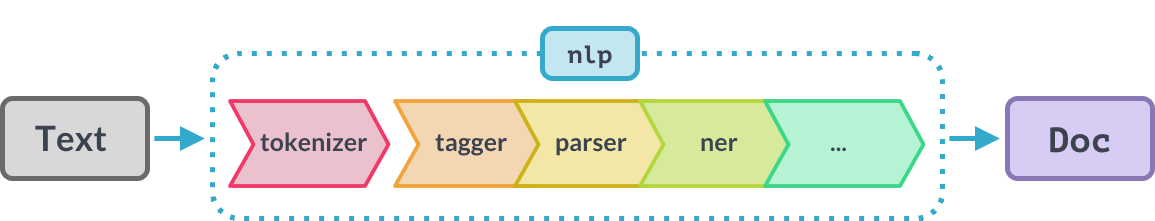
\includegraphics[scale=0.35]{../7-pictures/spacy_nlp_pipeline.png}
	\end{center}
\end{frame}
%..................................................................
\begin{frame}{Extracting Information from Text: Using spaCy}

\begin{itemize}
\item The Doc is then processed in several different steps – this is also referred to as the processing pipeline. 
\item The pipeline used by the trained pipelines typically include a tagger, a lemmatizer, a parser and an entity recognizer. Each pipeline component returns the processed Doc, which is then passed on to the next component.
\end{itemize}

	\begin{center}
	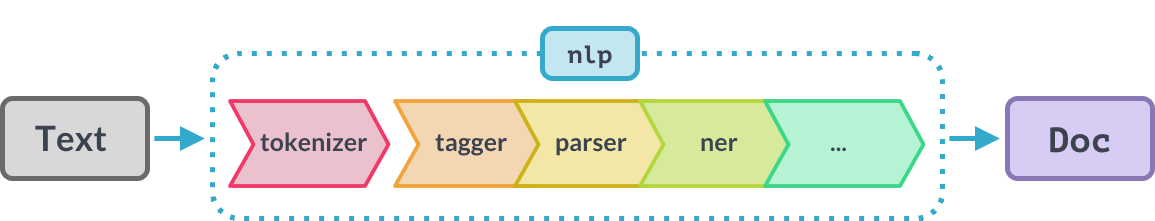
\includegraphics[scale=0.35]{../7-pictures/spacy_nlp_pipeline.png}
	\end{center}
\end{frame}
%..................................................................
\begin{frame}{Extracting Information from Text: Using spaCy}
	\begin{center}
	\includegraphics[scale=0.35]{../7-pictures/09_information_extraction_pic_5.png}
	\end{center}
\end{frame}
%..................................................................
\begin{frame}{\small Extracting Information from Text: Using NLTK with Stanford NER}
	\begin{center}
	\includegraphics[scale=0.35]{../7-pictures/stanford_ner_0.png}
	\end{center}
\end{frame}
%..................................................................
\begin{frame}{Example : Reading the Newspaper }
\begin{columns}[T] % align columns
\begin{column}{.48\textwidth}
        \begin{itemize}
		\item Notebook: \textbf{chapter-4-1}
		\item Libraries: NLTK, Stanford Group NER
		\item https://nlp.stanford.edu/software/
        \end{itemize}
\end{column}%
\hfill%
\begin{column}{.48\textwidth}
    %\fbox{
        \includegraphics[width=\linewidth]{../7-pictures/09_information_extraction_pic_6.png}
    %}
\end{column}%
\end{columns}
\end{frame}
%..................................................................
\begin{frame}{Comparing Results}

\begin{itemize}
\item Natural language processing applications are characterized by complex interdependent decisions that require large amounts of prior knowledge. 
\item In this case, as you can see, the system designed by Stanford did not achieve the same result as spaCy, but it is pure accident; in fact, a lot depends on how well the models have been trained and with how much data. 
\item For this reason, in case there is a need to perform a task like this, the best thing to do is to use multiple tools and compare the results, in order to find the best one in terms of performance and response.
\end{itemize}
\end{frame}

%---------------------------------------------------------------------------------------------------
\section{Text Vectorization \\ \scalebox{0.8}{Turning Words into Numbers}}
%---------------------------------------------------------------------------------------------------

\begin{frame}{Introduction}
	\begin{itemize}
		\item Machine learning algorithms operate on a numeric feature space, expecting input as a two-dimensional array where rows are instances and columns are features. 
		\item \highlight{\text{What are the appropriate features for applying a ML model to a}} \highlight{\text{text?}} 
		\item In order to perform machine learning on text, we need to transform our documents into vector representations such that we can apply numeric machine learning. 
		\item This process is called \textbf{feature extraction} or more simply, \textbf{vectorization}, and is an essential first step toward language-aware analysis.
	\end{itemize}
\end{frame}
%..................................................................
\begin{frame}{Introduction}
	\begin{itemize}
		\item For this reason, we must now make a critical shift in how we think about language - from a sequence of words to \highlight{\text{points that occupy a high-dimensional semantic space}}
	\end{itemize}
	\begin{center}
	\includegraphics[scale=0.4]{../7-pictures/06_text_vectorization_pic_0.png}
	\end{center}
\end{frame}
%..................................................................
\begin{frame}{Introduction}
	\begin{itemize}
		\item Points in space can be close together or far apart, tightly clustered or evenly distributed. 
		\item Semantic space is therefore mapped in such a way where documents with similar meanings are closer together and those that are different are farther apart. 
		\item By encoding \textbf{similarity} as distance, we can begin to derive the primary components of documents and draw decision boundaries in our semantic space.
		\item The simplest encoding of semantic space is the bag-of-words model, whose primary insight is that \highlight{\text{meaning and similarity are encoded in}} \highlight{\textbf{vocabulary}}.
	\end{itemize}
\end{frame}
%..................................................................
\subsection{Bag-of-Words (BOW) \\ \scalebox{0.8}{}}
%---------------------------------------------------------------------------------------------------
\begin{frame}{Bag-of-Words}
	\begin{itemize}
		\item To vectorize a corpus with a bag-of-words (BOW) approach, \textbf{we represent every document from the corpus as a vector whose length is equal to the vocabulary of the corpus}.
		\item The vocabulary is the set of words without repetition present in the whole corpus
	\end{itemize}
	\begin{center}
	\includegraphics[scale=0.6]{../7-pictures/06_text_vectorization_pic_1.png}
	\end{center}
	\footnotesize{image source: \textit{Bengfort B. et al. Text Analysis with Python}}
\end{frame}
%..................................................................
\begin{frame}{Bag-of-Words}
What should each element in the document vector be?
	\begin{itemize}
		\item We will explore several choices, each of which extends or modifies the base bag-of-words model to describe semantic space. 
		\item We will look at three types of vector encoding - frequency, one-hot, TF-IDF, - and discuss their implementations in Scikit-Learn and NLTK.
	\end{itemize}
	\begin{center}
	\includegraphics[scale=0.6]{../7-pictures/06_text_vectorization_pic_2.png}
	\end{center}
	\footnotesize{image source: \textit{Bengfort B. et al. Text Analysis with Python}}
\end{frame}
%..................................................................
\begin{frame}{Bag-of-Words}
	\begin{itemize}
		\item \textbf{Frequency Vectors}
		\item The simplest vector encoding model is to simply fill in the vector with \textbf{the frequency of each word as it appears in the document};
		\item In this encoding scheme each document is represented as the multiset of the tokens that compose it and the value for each word position in the vectr is its count;
		\item This representation can either be a straight count encoding or a normalized encoding where each word is weighted by the total number of words in the document;
	\end{itemize}
\end{frame}
%..................................................................
\begin{frame}{Bag-of-Words}
	Token Frequency as Vector Encoding
	\begin{center}
	\includegraphics[scale=0.6]{../7-pictures/06_text_vectorization_pic_3.png}
	\end{center}
	\footnotesize{image source: \textit{Bengfort B. et al. Text Analysis with Python}}
\end{frame}
%..................................................................
\begin{frame}{Text Feature Extraction}
	\begin{itemize}
		\item CountVectorizer: turns a collection of text documents into numerical feature vectors.
	\begin{center}
	\includegraphics[scale=0.5]{../7-pictures/06_text_vectorization_pic_5.png}
	\end{center}
		\item \textbf{TF}: Just counting the number of words in each document has 1 issue: it will give \textbf{more weightage to longer documents than shorter documents}. To avoid this, we can use frequency (\textbf{TF - Term Frequencies}) i.e. \#count(word) / \#Total words, in each document.
	\end{itemize}
\end{frame}
%..................................................................
\begin{frame}{Bag-of-Words  }
	\begin{center}
	\includegraphics[scale=0.5]{../7-pictures/06_text_vectorization_pic_4.png}
	\end{center}
\end{frame}
%..................................................................
\begin{frame}{One-Hot Encoding}
	One-Hot encoding is a method that produces a boolean vector. A particular vector index is marked as TRUE (1) if the token exist in the document and FALSE (0) if it does not.
	\begin{center}
	\includegraphics[scale=0.5]{../7-pictures/06_text_vectorization_pic_6.png}
	\end{center}
	\footnotesize{image source: \textit{Bengfort B. et al. Text Analysis with Python}}
\end{frame}
%..................................................................
\begin{frame}{Term Frequency-Inverse Document Frequency }
	\begin{itemize}
		\item The bag-of-words representations that we have explored so far only describe a document in a standalone fashion, \textbf{not taking into account the context of the corpus}. 
		\item A better approach would be to consider the \textbf{relative frequency or rareness of tokens in the document against their frequency in other documents}. 
		\item The central insight is that \textbf{meaning is most likely encoded in the more rare terms from a document}.
	\end{itemize}
\end{frame}
%..................................................................
\begin{frame}{Compute Inverse Document Frequency}
	\begin{itemize}
		\item The inverse document frequency is a measure of how much information the word provides, that is, whether the term is common or rare across all documents. 
		\item It is the logarithmically scaled inverse fraction of the documents that contain the word, obtained by dividing the total number of documents by the number of documents containing the term, and then taking the logarithm of that quotient: 
		\begin{equation}idf(t,D) = \log \frac{N}{\vert \{  d \in D: t \in d\}\vert} 
		\end{equation}  
		where \textbf{the numerator ($N$) is the total number of documents} in the corpus and \textbf{the denominator is the number of documents where the term $t$ appears}.
	\end{itemize}
\end{frame}
%..................................................................
\begin{frame}{Compute Inverse Document Frequency}
	\begin{center}
	\includegraphics[scale=0.45]{../7-pictures/06_text_vectorization_pic_8.png}
	\end{center}
\end{frame}
%..................................................................
\begin{frame}{Term Frequency-Inverse Document Frequency }
	\begin{itemize}
		\item TF-IDF, term frequency-inverse document frequency, encoding normalizes the frequency of tokens in a document with respect to the rest of the corpus. 
		\item This encoding approach accentuates terms that are very relevant to a specific instance, as shown in Figure, where the token studio has a higher relevance to this document since it only appears there.
	\end{itemize}
	\begin{center}
	\includegraphics[scale=0.5]{../7-pictures/06_text_vectorization_pic_7.png}
	\end{center}
	\footnotesize{image source: \textit{Bengfort B. et al. Text Analysis with Python}}
\end{frame}
%..................................................................
\begin{frame}{Compute Term Frequency-Inverse Document Frequency}
	\begin{itemize}
		\item Then tf-idf is calculated as: \begin{equation} tfidf(t,d,D) = tf(t,d) \cdot idf(t,D)\end{equation}
		\item A high weight in tf-idf is reached by a \highlight{\text{high term frequency}} (in the given document) and a \highlight{\text{low document frequency}} of the term in the whole collection of documents; 
\item The weights hence tend to filter out common terms. 
		\item Since the ratio inside the idf's log function is always greater than or equal to 1, the value of idf (and tf-idf) is greater than or equal to 0. As a term appears in more documents, the ratio inside the logarithm approaches 1, bringing the idf and tf-idf closer to 0.
	\end{itemize}
\end{frame}
%..................................................................
\begin{frame}{Compute Term Frequency-Inverse Document Frequency}
	\begin{center}
	\includegraphics[scale=0.5]{../7-pictures/06_text_vectorization_pic_9.png}
	\end{center}
\end{frame}
%..................................................................
\begin{frame}{Text Feature Extraction}
	CountVectorizer: turns a collection of text documents into numerical feature vectors.
	\begin{center}
	\includegraphics[scale=0.5]{../7-pictures/06_text_vectorization_pic_10.png}
	\end{center}
	As tf-idf is very often used for text features, there is also another class called TfidfVectorizer that combines all the options of CountVectorizer and TfidfTransformer in a single model
	\begin{center}
	\includegraphics[scale=0.5]{../7-pictures/06_text_vectorization_pic_11.png}
	\end{center}
\end{frame}
%..................................................................
\begin{frame}{Document Similarity}
	\begin{itemize}
		\item When you have vectorized your text, we can try to define a distance metric such that documents that are closer together in feature space are more similar.
		\item There are a number of different measures that can be used to determine document similarity; 
	\end{itemize}
	\begin{center}
	\includegraphics[scale=0.4]{../7-pictures/06_text_vectorization_pic_12.png}
	\end{center}
\end{frame}
%..................................................................
\begin{frame}{Document Similarity}
	\begin{itemize}
		\item Fundamentally, each relies on our ability to imagine documents as points in space, where the relative closeness of any two documents is a measure of their similarity.
	\end{itemize}
	\begin{center}
	\includegraphics[scale=0.4]{../7-pictures/06_text_vectorization_pic_13.png}
	\end{center}
\end{frame}
%..................................................................
\begin{frame}{Document Similarity}
\begin{columns}[T] % align columns
\begin{column}{.48\textwidth}
        \begin{itemize}
		\item We can measure vector similarity with cosine distance, using the cosine of the angle between the two vectors to assess the degree to which they share the same orientation. 
		\item In effect, the more parallel any two vectors are, the more similar the documents will be (regardless of their magnitude).
        \end{itemize}
\end{column}%
\hfill%
\begin{column}{.48\textwidth}
    %\fbox{
        \includegraphics[width=\linewidth]{../7-pictures/06_text_vectorization_pic_14.png}
    %}
\end{column}%
\end{columns}
\end{frame}
\begin{frame}{Document Similarity}
	\begin{itemize}
		\item Mathematically, Cosine similarity metric measures the cosine of the angle between two n-dimensional vectors projected in a multi-dimensional space. The Cosine similarity of two documents will range from 0 to 1. If the Cosine similarity score is 1, it means two vectors have the same orientation. The value closer to 0 indicates that the two documents have less similarity.
		\item The mathematical equation of Cosine similarity between two non-zero vectors is: \begin{equation} \text{similarity} = \cos(\theta) = \frac{\mathbf{A} \cdot \mathbf{B}}{\left\Vert\mathbf{A}\right\Vert \,\left\Vert\mathbf{B}\right\Vert} = \frac{\sum\limits_{i=1}^n A_iB_i}{\sum\limits_{i=1}^n A_i^2 \sum\limits_{i=1}^n B_i^2} \end{equation}
	\end{itemize}
\end{frame}
%..................................................................
\begin{frame}{Example : Bag-of-Words}
\begin{columns}[T] % align columns
\begin{column}{.48\textwidth}
        \begin{itemize}
		\item Notebook: \textbf{chapter-4-2}
		\item Focus: Vectorization with sklearn, Document Similarity
		\item Libraries: NLTK, sklearn
        \end{itemize}
\end{column}%
\hfill%
\begin{column}{.48\textwidth}
    %\fbox{
        \includegraphics[width=\linewidth]{../7-pictures/09_information_extraction_pic_6.png}
    %}
\end{column}%
\end{columns}
\end{frame}
%..................................................................
\subsection{Word Embedding \\ \scalebox{0.8}{}}
%---------------------------------------------------------------------------------------------------
\begin{frame}{What is Word Embedding}
	\begin{itemize}
		\item The different encoding we have discussed so far is arbitrary as \textbf{it does not capture any relationship between words}. 
		\item It can be challenging for a model to interpret, for example, a linear classifier learns a single weight for each feature. 
		\item Because there is no relationship between the similarity of any two words and the similarity of their encodings, this feature-weight combination is not meaningful.
		\item Furthermore, \textbf{the dimension of the vector space}, being equal to the number of terms in the vocabulary, \textbf{tends to increase considerably} as the size of the corpus increases.
	\end{itemize}
\end{frame}
%..................................................................
\begin{frame}{What is Word Embedding}
\begin{columns}[T] % align columns
\begin{column}{.48\textwidth}
        \begin{itemize}
        \item Relationship between words
		\item For example, we humans understand the words like king and queen, man and woman, tiger and tigress have a certain type of relation between them but how can a computer figure this out?
        \end{itemize}
\end{column}%
\hfill%
\begin{column}{.48\textwidth}
    %\fbox{
        \includegraphics[width=\linewidth]{../7-pictures/06_text_vectorization_pic_15.png}
    %}
\end{column}%
\end{columns}
\end{frame}
%..................................................................
\begin{frame}{What is Word Embedding}
\begin{columns}[T] % align columns
\begin{column}{.48\textwidth}
        \begin{itemize}
		\item It should be nice to have representations of text in an n-dimensional space where \highlight{\text{words that have the same}} 
\highlight{\text{meaning have a similar}} 
\highlight{\text{representation}}. 
		\item Meaning that two similar words are represented by almost similar vectors that are very closely placed in a vector space. 
        \end{itemize}
\end{column}%
\hfill%
\begin{column}{.48\textwidth}
    %\fbox{
        \includegraphics[width=\linewidth]{../7-pictures/06_text_vectorization_pic_16.png}
    %}
\end{column}%
\end{columns}
\end{frame}
%..................................................................
\begin{frame}{What is Word Embedding}
\begin{columns}[T] % align columns
\begin{column}{.48\textwidth}
        \begin{itemize}
		\item Thus when using word embeddings, all individual words are represented as real-valued vectors in a predefined vector space. 
		\item Each word is mapped to one vector and the vector values are learned in a way that resembles a neural network.
        \end{itemize}
\end{column}%
\hfill%
\begin{column}{.48\textwidth}
    %\fbox{
        \includegraphics[width=\linewidth]{../7-pictures/06_text_vectorization_pic_17.png}
    %}
\end{column}%
\end{columns}
%..................................................................
\end{frame}
\begin{frame}{The Importance of Context}
	\begin{itemize}
		\item The concept of embeddings arises from a branch of Natural Language Processing called - \textit{Distributional Semantics}. It is based on the simple intuition that:
		\item \textbf{Words that occur in similar contexts tend to have similar meanings.}
		\item In other words, a word meaning is given by the words that it appears frequently with.
	\end{itemize}
	
\begin{tcolorbox}
Conceptually it involves the mathematical embedding \textbf{from space with many dimensions} per word to a \textbf{continuous vector space with a much lower dimension}.
\end{tcolorbox}

\end{frame}
%..................................................................
\begin{frame}{What is Word2Vec?}
	\begin{itemize}
		\item Word2vec is a method to efficiently create word embeddings by using a two-layer neural network.  
		\item It was developed by Tomas Mikolov, et al. at Google in 2013 as a response to make the neural-network-based training of the embedding more efficient and since then has become the de facto standard for developing pre-trained word embedding. 		  
		\item The input of word2vec is a text corpus and its output is a set of vectors known as feature vectors that represent words in that corpus. 
		
	\end{itemize}
\end{frame}
%..................................................................
\begin{frame}{Word2Vec}
	\begin{itemize}
	\item The Word2Vec objective function causes the words that have a similar context to have similar embeddings. 
		\item Thus in this vector space, these words are really close. Mathematically, the cosine of the angle (Q) between such vectors should be close to 1, i.e. angle close to 0.
		\item Word2vec is not a single algorithm but a combination of two techniques - CBOW(Continuous bag of words) and Skip-gram model.
		\item Both these are shallow neural networks which map word(s) to the target variable which is also a word(s). 
		\item Both these techniques learn weights which act as word vector representations. 
	\end{itemize}
\end{frame}
%..................................................................
\begin{frame}{Word2Vec : CBOW approach}
	\begin{itemize}
		\item CBOW predicts the probability of a word to occur \textbf{given the words surrounding it}. We can consider a single word or a group of words. But for simplicity, we will take a single context word and try to predict a single target word.
		\item The English language contains almost 1.2 million words, making it impossible to include so many words in our example. So I will consider a small example in which we have only four words i.e. \textbf{live}, \textbf{home}, \textbf{they} and \textbf{at}. For simplicity, we will consider that the corpus contains only one sentence, that being, \textbf{They live at home}.
	\end{itemize}
\end{frame}
%..................................................................
\begin{frame}{Word2Vec : CBOW approach}
	First, we convert each word into a one-hot encoding form. Also, we will not consider all the words in the sentence but ll only take certain words that are in a window. 
	\begin{center}
	\includegraphics[scale=0.4]{../7-pictures/06_text_vectorization_pic_18.png}
	\end{center}
	\footnotesize{image source: \textit{https://www.mygreatlearning.com/blog/word-embedding/}}
\end{frame}
%..................................................................
\begin{frame}{Word2Vec : CBOW approach}
	For example, for a window size equal to three, we only consider three words in a sentence. The middle word is to be predicted and the surrounding two words are fed into the neural network as context. The window is then slide and the process is repeated again.
	\begin{center}
	\includegraphics[scale=0.4]{../7-pictures/06_text_vectorization_pic_19.png}
	\end{center}
	\footnotesize{image source: \textit{https://www.mygreatlearning.com/blog/word-embedding/}}
\end{frame}
%..................................................................
\begin{frame}{Word2Vec : CBOW approach}
	\begin{itemize}
		\item Finally, after training the network repeatedly by sliding the window a shown above, we get weights which we use to get the embeddings as shown below.
		\item Usually, we take a window size of around 8-10 words and have a vector size of 300.
	\end{itemize}
	\begin{center}
	\includegraphics[scale=0.5]{../7-pictures/06_text_vectorization_pic_20.png}
	\end{center}
	\footnotesize{image source: \textit{https://www.mygreatlearning.com/blog/word-embedding/}}
\end{frame}
%..................................................................
\begin{frame}{Word2Vec : Skip-Gram Model}
	\begin{itemize}
		\item The Skip-gram model tries to predict the source context words (surrounding words) given a target word (the centre word)
		\item The working is conceptually similar to the CBOW, there is just a difference in the architecture of its NN and in the way the weight matrix is generated:	 
	\end{itemize}
	\begin{center}
	\includegraphics[scale=0.4]{../7-pictures/06_text_vectorization_pic_21.png}
	\end{center}
	\footnotesize{image source: \textit{https://www.mygreatlearning.com/blog/word-embedding/}}
\end{frame}
%..................................................................
\begin{frame}{Example : Word2Vec}
\begin{columns}[T] % align columns
\begin{column}{.48\textwidth}
        \begin{itemize}
		\item Notebook: \textbf{chapter-4-2}
		\item Focus: Implementing a word2vec model using a CBOW NN architecture
		\item Libraries: NLTK, keras
        \end{itemize}
\end{column}%
\hfill%
\begin{column}{.48\textwidth}
    %\fbox{
        \includegraphics[width=\linewidth]{../7-pictures/09_information_extraction_pic_6.png}
    %}
\end{column}%
\end{columns}
\end{frame}
%---------------------------------------------------------------------------------------------------
\section{Text Classification}
%---------------------------------------------------------------------------------------------------
\begin{frame}{Introduction}
	\begin{itemize}
		\item Text Classification is the process of labeling or organizing text data into groups - it forms a fundamental part of Natural Language Processing.
		\item In the digital age that we live in, we are surrounded by text on our social media accounts, commercials, websites, Ebooks, etc. The majority of this text data is \textbf{unstructured}, so classifying this data can be extremely useful.
		\item The premise of classification is simple: given a categorical target variable, learn patterns that exist between instances composed of independent variables and their relationship to the target. 
	\end{itemize}
\end{frame}
%..................................................................
\begin{frame}{Introduction}
\textbf{Text Classification: a formal definition}\\
\vspace{0.5cm}
\textbf{INPUT}:
\begin{itemize}
\item a document $d$;
\item a fixed set of classes $C=\{C_1, C_2, \dots, C_n \}$
\end{itemize}
\vspace{0.5cm}
\textbf{OUTPUT}
\begin{itemize}
\item a predicted class $c \in C$
\end{itemize}
\end{frame}
%..................................................................
\begin{frame}{Introduction}
	Text Classification has a wide array of applications. Some popular uses are:
	\begin{itemize}
		\item Spam detection in emails
		\item Sentiment analysis of online reviews
		\item Topic labeling documents like research papers
		\item Language detection like in Google Translate
		\item Age/gender identification of anonymous users
		\item Tagging online content
		\item Speech recognition used in virtual assistants (like Siri and Alexa)
	\end{itemize}
\end{frame}
%..................................................................
\begin{frame}{Introduction}
\textbf{Hand-coded rules}
\vspace{0.5cm}
\begin{itemize}
\item Rules based on combinations of words or other features, for example:
 spam if black-list-address OR (“dollars” AND “you have been selected”)
\item Accuracy can be high if rules carefully refined by expert
\item But building and maintaining these rules is expensive

\end{itemize}
\end{frame}
%..................................................................
\begin{frame}{Introduction}
	\begin{itemize}
		\item Because \textbf{the target is given ahead of time}, classification is a \highlight{\text{supervised}} machine learning model because a model can be trained to minimize error between predicted and actual categories in the training data. 
		\item Once a classification model is fit, it assigns categorical labels to new instances based on the patterns detected during training.
		\item The application problem can be formulated to identify either a yes/no (binary classification) or discrete buckets (multiclass classification).
	\end{itemize}
\end{frame}
%..................................................................
\begin{frame}{Introduction}
\textbf{Text Classification: Supervised Machine Learning}\\
\vspace{0.5cm}
\textbf{INPUT}:
\begin{itemize}
\item a document $d$;
\item a fixed set of classes $C=\{C_1, C_2, \dots, C_n \}$
\item a training set of $m$ hand-labeled documents $(d_1,c_1), \dots,(d_m,c_m)$
\end{itemize}
\vspace{0.5cm}
\textbf{OUTPUT}
\begin{itemize}
\item a learned classifier $\gamma:d \rightarrow c$
\end{itemize}
\end{frame}
%..................................................................
\begin{frame}{Introduction}
All classifier model families have the same basic workflow, and with Scikit-Learn Estimator objects, they can be employed in a procedural fashion and compared using cross-validation to select the best performing predictor.
The classification workflow occurs in two phases: a build phase and an operational phase.
	\begin{itemize}
		\item In the build phase, a corpus of documents is transformed into feature vectors. The document features, along with their annotated labels (the category or class we want the model to learn), are then passed into a classification algorithm that defines its internal state along with the learned patterns. 
		\item Once trained or fitted, a new document can be vectorized into the same space as the training data and passed to the predictive algorithm, which returns the assigned class label for the document.
	\end{itemize}
\end{frame}
%..................................................................
\begin{frame}{Introduction}
	\begin{center}
	\includegraphics[scale=0.8]{../7-pictures/07_classification_for_text_analysis_pic_0.png}
	\end{center}
	\footnotesize{source: \textit{Bengfort B. et al. Text Analysis with Python}}
\end{frame}
%..................................................................
\begin{frame}{Example 1 - Gender Identification}
In this first example we will try to build a simple algorithm to understand if a noun passed in input is of masculine or feminine gender. In this, and in the following examples, we will implicitly assume that the language used is English.
\\
\vspace{0.5cm}
\textbf{FOCUS}
\\
	\begin{itemize}
		\item How build a feature in text analysis
		\item Training Vs validation
	\end{itemize}
\end{frame}
%..................................................................
\begin{frame}{Example 2 - The \textit{20 Newsgroup} data set}
	\begin{itemize}
		\item In this example we are going to work with the "20 Newsgroup Dataset". 
		\item The 20 Newsgroups data set is a collection of approximately 20,000 newsgroup documents, partitioned (nearly) evenly across 20 different newsgroups. The 20 newsgroups collection has become a popular data set for experiments in text applications of machine learning techniques, such as text classification and text clustering. 
		\item This data set is infact in-built in scikit, so we don’t need to download it explicitly.
	\end{itemize}
\end{frame}
%..................................................................
\begin{frame}{Example 2 - The \textit{20 Newsgroup} data set}
	\textbf{FOCUS}
	\vspace{0.5cm}
	\begin{itemize}
		\item using sklearn package
		\item numerical features and vectorization process
		\item building a ml pipeline with sklearn
		\item model optimization
	\end{itemize}
\end{frame}
%..................................................................
\begin{frame}{Example : Text Classification}
\begin{columns}[T] % align columns
\begin{column}{.48\textwidth}
        \begin{itemize}
		\item Notebook: \textbf{chapter-4-3}
		\item Libraries: NLTK, keras
        \end{itemize}
\end{column}%
\hfill%
\begin{column}{.48\textwidth}
    %\fbox{
        \includegraphics[width=\linewidth]{../7-pictures/09_information_extraction_pic_6.png}
    %}
\end{column}%
\end{columns}
\end{frame}

%..................................................................
\subsection{Sentiment Analysis with Keras \\ \scalebox{0.8}{From \textit{Deep Learning with Python by F. Chollet}}}
%---------------------------------------------------------------------------------------------------
\begin{frame}{Sentiment Analysis with Keras}
	\begin{itemize}
		\item The IMDb Movie Reviews dataset is a binary sentiment analysis dataset consisting of 50,000 reviews from the Internet Movie Database (IMDb) labeled as positive or negative. 
		\item The dataset contains an even number of positive and negative reviews. 
		\item Only highly polarizing reviews are considered. 
		\item A negative review has a score = 4 out of 10, and a positive review has a score = 7 out of 10. 
		\item No more than 30 reviews are included per movie. 
		\item The dataset contains additional unlabeled data.
	\end{itemize}
\end{frame}
%..................................................................
\begin{frame}{The IMDb Movie Reviews Dataset}
	\begin{itemize}
		\item Just like the MNIST dataset, the IMDB dataset comes packaged with Keras. 
		\item It has already been preprocessed: the reviews (sequences of words) have been turned into sequences of integers, where each integer stands for a specific word in a dictionary.
		\item The following code will load the dataset (when you run it the first time, about 80 MB of data will be downloaded to your machine).
	\end{itemize}
	\begin{center}
	\includegraphics[scale=0.5]{../7-pictures/07_classification_for_text_analysis_pic_3.png}
	\end{center}
\end{frame}
%..................................................................
\begin{frame}{The IMDb Movie Reviews Dataset}
	\begin{itemize}
		\item \textbf{One-hot encode}
		\item All lists are transformed into vectors of 0s and 1s. 
		\item This would mean, for instance, turning the sequence [3, 5] into a 10,000-dimensional vector that would be all 0s except for indices 3 and 5, which would be 1s. 
		\item Then you could use as the first layer in your network a Dense layer, capable of handling floating-point vector data.
	\end{itemize}
	\begin{center}
	\includegraphics[scale=0.5]{../7-pictures/07_classification_for_text_analysis_pic_4.png}
	\end{center}
\end{frame}
%..................................................................
\begin{frame}{Preparing the data}
	\begin{itemize}
		\item The input data is vectors, and the labels are scalars (1s and 0s). 
		\item A type of network that performs well on such a problem is a simple stack of fully connected (Dense) layers with relu activations.
		\item The argument being passed to each Dense layer (16) is the number of hidden units of the layer.
		\item The intermediate layers will use relu as their activation function, and the final layer will use a sigmoid activation so as to output a probability (a score between 0 and 1, indicating how likely the review is to be positive). 
	\end{itemize}
\end{frame}
%..................................................................
\begin{frame}{Building our Network}
	\begin{center}
	\includegraphics[scale=0.35]{../7-pictures/07_classification_for_text_analysis_pic_5.png}
	\end{center}
\end{frame}
%..................................................................
\begin{frame}{Building our Network}
	\begin{center}
	\includegraphics[scale=0.4]{../7-pictures/07_classification_for_text_analysis_pic_6.png}
	\end{center}
\end{frame}
%..................................................................
\begin{frame}{Building our Network}
	\begin{itemize}
		\item Finally, we need to choose a loss function and an optimizer. 
		\item Because we are facing a binary classification problem and the output of your network is a probability (we end our network with a single-unit layer with a sigmoid activation), it is best to use the binary\_crossentropy loss. 
		\item It is not the only viable choice: you could use, for instance, the well known mean squared error but crossentropy is usually the best choice when you're dealing with models that output probabilities. 
		\item Crossentropy is a quantity from the field of Information Theory that measures the distance between probability distributions or, in this case, between the ground-truth distribution and your predictions.
	\end{itemize}
\end{frame}
%..................................................................
\begin{frame}{Loss Function and Optimizer}
	\begin{itemize}
		\item \textbf{RMSprop} is unpublished optimization algorithm designed for neural networks, first proposed by Geoff Hinton in lecture 6 of the online course \textbf{Neural Networks for Machine Learning};
		\item \textbf{Adaptive learning rate} methods are an optimization of gradient descent methods with the goal of minimizing the objective function of a network by using the gradient of the function and the parameters of the network.
	\end{itemize}
	\begin{center}
	\includegraphics[scale=0.5]{../7-pictures/07_classification_for_text_analysis_pic_7.png}
	\end{center}
\end{frame}
%..................................................................
\begin{frame}{Example}
\begin{columns}[T] % align columns
\begin{column}{.48\textwidth}
        \begin{itemize}
		\item Now that we have described the construction of the neural network, let's see how it works in practice ...
		\item Using \textbf{chollet-deep-learning-with-python-sentiment} Notebook 
        \end{itemize}
\end{column}%
\hfill%
\begin{column}{.48\textwidth}
    %\fbox{
        \includegraphics[width=\linewidth]{../7-pictures/07_classification_for_text_analysis_pic_8.png}
    %}
\end{column}%
\end{columns}
\end{frame}

%---------------------------------------------------------------------------------------------------
\section{Clustering for Text Similarity \\ \scalebox{0.8}{Sorting Documents}}
%---------------------------------------------------------------------------------------------------
\begin{frame}{Similarity}
	\begin{itemize}
		\item At its core, any sorting task relies on our ability to compare two documents and determine their \textbf{SIMILARITY}. 
	\end{itemize}
	\begin{center}
	\includegraphics[scale=0.5]{../7-pictures/08_clustering_for_text_similarity_pic_0.png}
	\end{center}
\end{frame}
%..................................................................
\begin{frame}{Introduction}
\begin{columns}[T] % align columns
\begin{column}{.48\textwidth}
        \begin{itemize}
		\item Documents that are similar to each other are grouped together and the resulting groups broadly describe the overall themes, topics, and patterns inside the corpus.
        \end{itemize}
\end{column}%
\hfill%
\begin{column}{.48\textwidth}
    %\fbox{
        \includegraphics[width=\linewidth]{../7-pictures/08_clustering_for_text_similarity_pic_1.png}
    %}
\end{column}%
\end{columns}
\end{frame}
\begin{frame}{Introduction}
\begin{columns}[T] % align columns
\begin{column}{.48\textwidth}
        \begin{itemize}
		\item While most document sorting is currently done manually, it is possible to achieve these tasks in a fraction of the time with the effective integration of unsupervised learning, as we will see in this lesson
        \end{itemize}
\end{column}%
\hfill%
\begin{column}{.48\textwidth}
    %\fbox{
        \includegraphics[width=\linewidth]{../7-pictures/08_clustering_for_text_similarity_pic_2.png}
    %}
\end{column}%
\end{columns}
\end{frame}
\begin{frame}{Introduction}
	\begin{itemize}
		\item In many situations, corpora do not arrive \textit{pretagged} with labels ready for classification. 
		\item In these cases, the only choice, or at least a necessary precursor for many natural language processing tasks, is an unsupervised approach. 
		\item Clustering algorithms aim to discover \textbf{latent structure} or themes in unlabeled data using features to organize instances into meaningfully dissimilar groups.
		\item With text data, each \textbf{ instance} is a single document or sentence, and the \textbf{features} are its tokens, vocabulary, structure, metadata, etc.
	\end{itemize}
\end{frame}
%..................................................................
\begin{frame}{Unsupervised Learning on Text}
	\begin{itemize}
		\item \textbf{Comparison between Clustering and Classification}
		\item The behavior of unsupervised learning methods is fundamentally different from that of supervised algorithm we have seen in the previous section; 
		\item \textbf{Instead of learning a predefined pattern, the model attempts to find relevant patterns a priori}.
		\item A clustering algorithm is usually employed to create groups or topic clusters, using a \underline{distance metric} such that documents that are closer together in feature space are more similar. 
		\item New incoming documents can then be vectorized and assigned to the nearest cluster.
	\end{itemize}
\end{frame}
%..................................................................
\begin{frame}{Unsupervised Learning on Text}
\begin{columns}[T] % align columns
\begin{column}{.48\textwidth}
        \begin{itemize}
		\item A corpus is transformed into feature vectors and a clustering algorithm is employed to create groups or topic clusters, using a distance metric such that documents that are closer together in feature space are more similar. 
		\item New incoming documents can then be vectorized and assigned to the nearest cluster.
        \end{itemize}
\end{column}%
\hfill%
\begin{column}{.48\textwidth}
    %\fbox{
        \includegraphics[width=\linewidth]{../7-pictures/08_clustering_for_text_similarity_pic_3.png}
    %}
\end{column}%
\end{columns}
\end{frame}
\begin{frame}{Unsupervised Learning on Text}
	\begin{itemize}
		\item As we have seen in section 3.1, there are a number of different measures that can be used to determine document similarity; 
		\item Remember that, fundamentally, each relies on our ability to imagine documents as points in space, where the relative closeness of any two documents is a measure of their similarity.
		\item We have discussed the \textbf{cosine similarity} but there are others measure of distance we can use in clustering documents. 
	\end{itemize}
\end{frame}
%..................................................................
\begin{frame}{Unsupervised Learning on Text : Similarity}
	\begin{center}
	\includegraphics[scale=0.4]{../7-pictures/08_clustering_for_text_similarity_pic_4.png}
	\end{center}
\end{frame}
%..................................................................
\begin{frame}{Document Similarity}
\begin{columns}[T] % align columns
\begin{column}{.48\textwidth}
        \begin{itemize}
		\item We can measure vector similarity with cosine distance, using the cosine of the angle between the two vectors to assess the degree to which they share the same orientation. 
		\item In effect, the more parallel any two vectors are, the more similar the documents will be (regardless of their magnitude).
        \end{itemize}
\end{column}%
\hfill%
\begin{column}{.48\textwidth}
    %\fbox{
        \includegraphics[width=\linewidth]{../7-pictures/08_clustering_for_text_similarity_pic_5.png}
    %}
\end{column}%
\end{columns}
\end{frame}
\subsection{Clustering \\ \scalebox{0.8}{}}
%---------------------------------------------------------------------------------------------------
\begin{frame}{Clustering}
	\begin{itemize}
		\item Now that we can quantify the similarity between any two documents, we can begin exploring unsupervised methods for finding similar groups of documents. 
		\item \textbf{Partitive clustering} and \textbf{agglomerative clustering} are our two main approaches, and both separate documents into groups whose members share maximum similarity as defined by some distance metric.
		\item \textbf{We will focus on partitive methods, which partition instances into groups that are represented by a central vector (the centroid)} or described by a density of documents per cluster. 
		\item Centroids represent an aggregated value (e.g., mean or median) of all member documents and are a convenient way to describe documents in that cluster.
	\end{itemize}
\end{frame}
%..................................................................
\begin{frame}{Clustering}
	\begin{itemize}
		\item As we have seen in the first part, clustering can be considered one of the most important unsupervised learning problem; so, as every other problem of this kind, it deals with finding a structure in a collection of unlabeled data. 
		\item A loose definition of clustering could be \textit{the process of organizing objects into groups whose members are similar in some way}. 
		\item A cluster is therefore a collection of objects which are coherent internally, but clearly dissimilar to the objects belonging to other clusters.
	\end{itemize}
\end{frame}
%..................................................................
\begin{frame}{Text Documents Clustering using K-Means Algorithm }
	\begin{center}
	\includegraphics[scale=0.5]{../7-pictures/08_clustering_for_text_similarity_pic_6.png}
	\end{center}
	\footnotesize{source: \textit{https://www.codeproject.com/Articles/439890/Text-Documents-Clustering-using-K-Means-Algorithm}}
\end{frame}
%..................................................................
\begin{frame}{Text Documents Clustering using K-Means Algorithm}
	\begin{itemize}
		\item \textbf{Document Representation}
		\item \highlight{\text{Each document is represented as a vector}} using the vector space model. 
		\item The vector space model also called term vector model is an algebraic model for representing text document (or any object, in general) as vectors of identifiers. \highlight{\text{For example, TF-IDF weight}}.
		\item \textbf{Finding Similarity Score}
		\item We will use cosine similarity to identify the similarity score of a document. 
	\end{itemize}
\end{frame}
%..................................................................
\begin{frame}{Text Documents Clustering using K-Means Algorithm}
	\begin{itemize}
		\item \textbf{A Practical Example: Clustering Movie Reviews}
		\item We are going to use data collected by Brandon Rose; 
		\item here the link to the original post: http://brandonrose.org/top100
		\item And the GitHub Repository in which you can find all the data files necessary for this example: https://github.com/brandomr/document\textunderscore cluster
	\end{itemize}
\end{frame}
%..................................................................
\begin{frame}{Text Documents Clustering using K-Means Algorithm}
	\textbf{5 Steps}
	\begin{itemize}
		\item Prepare data
		\item Tokenizing and stemming each synopsis
		\item Transforming the corpus into vector space using tf-idf
		\item Calculating cosine distance between each document as a measure of similarity
		\item Clustering the documents using the k-means algorithm
	\end{itemize}
\end{frame}
%..................................................................
\begin{frame}{Example : Clustering Document}
\begin{columns}[T] % align columns
\begin{column}{.48\textwidth}
        \begin{itemize}
		\item Notebook: \textbf{chapter-4-4}
		\item Libraries: NLTK, keras
        \end{itemize}
\end{column}%
\hfill%
\begin{column}{.48\textwidth}
    %\fbox{
        \includegraphics[width=\linewidth]{../7-pictures/09_information_extraction_pic_6.png}
    %}
\end{column}%
\end{columns}
\end{frame}

%=====================================================================


\end{document}
